\documentclass[11pt,a4paper,sans]{moderncv}

\moderncvstyle{casual}
\moderncvcolor{blue}

\usepackage[utf8]{inputenc}
\usepackage[T1]{fontenc}
\usepackage[french]{babel}

\newcommand\Colorhref[3][cyan]{\href{#2}{\small\color{#1}#3}}

\usepackage{xcolor}
\definecolor{quote}{HTML}{45376a}
\definecolor{author}{HTML}{5a4062}

\usepackage[scale=0.75]{geometry}
\graphicspath{{figures/}}

%%% personal data
\name{Vincent}{Lafouasse}
\title{Graduate research student in Molecular Chemistry (M2)}
\address{28 square du clos de Villaine}{91300 Massy}{\textsc{France}}
\phone[mobile]{+33 6 21 59 25 74}
\phone[fixed]{+33 9 50 40 28 82}
\email{vincent.lafouasse@universite-paris-saclay.fr}
\social[github]{vincent-lafouasse}
\social[linkedin]{vincent-lafouasse}
\social[twitter]{VLafouasse}

%-------------------------------------------------------------------------------
%            content
%-------------------------------------------------------------------------------
\begin{document}

\makecvtitle

%%% Quote
{
    \vspace{-5mm}
    \centering
    \color{quote}
    \rmfamily
    ``There is excitment, adventure, and challenge,\\
    and there can be great art in organic synthesis.''\\
}

\begin{flushright}
    {\color{author}
    {---}  \textsc{Robert B. Woodward}
    \footnote{as reported by: Nicolaou, K. C.; Sorensen, E. J. Introduction: Constructing the Molecules of Nature. \\
    In \textit{Classics in total synthesis: targets, strategies, methods}; Wiley-VCH ; \textbf{1996}; p 3.
}}
\end{flushright}
%
%
%
\section{Research Interest}
\cvitem{\textsc{About me}}{%
I am mainly interested in the field of Organic Synthesis, especially Total Synthesis.{\newline} %
I am currently looking for a 6-month internship beginning January 2021 %
and for a PhD for Fall 2021.}
%
%
%
\section{Education}
\cventry{Fall 2020}{(M2) M.Sc. Molecular Chemistry and Interfaces}%
{{\newline}École Normale Supérieure de Paris-Saclay -- École Polytechnique}%
{Paris-Saclay (91)}{}%
{A high-level program devoted to molecular chemistry and its applications %
to the fields of biology and material sciences. %
More information on the program \Colorhref[red]{https://www.ip-paris.fr/master-2-molecular-chemistry-and-interfaces/}{at this link}. %
\medbreak
$\bullet$ \textit{Curriculum}: Advanced organic synthesis, Organometallic chemistry and Catalysis, %
Supramolecular chemistry, Chemical Biology, %
Molecular modeling and chemistry for Optoelectronics.%
}
\vspace{5mm}
%
%
\cventry{2018--2020}{(M1) M.Sc. Chemistry}%
{Université Paris-Saclay}{Orsay (91)}{High Honours}%
{Organic Chemistry specialization}
%
%
\cventry{2017--2018}{(L3) B.Sc. Chem. (Physics minor)}%
{Sorbonne Université (ex-UPMC)}{Paris (75)}{High Honours}%
{Fundamentals of Chemistry and Physics}
%
%
\cventry{2015--2017}{B.Sc. Sciences de la Matière}%
{Ecole Normale Supérieure de Lyon}{Lyon (69)}{}%
{Élève normalien : A unique, non-specialized training program in Physics and Chemistry}
%
%
\cventry{2013--2015}{Classe Préparatoire PCSI/PC$^*$ (CPGE)}%
{Lycée Henri IV}{Paris (75)}{}%
{Two years of intensive theoretical courses in Mathematics, Physics and Chemistry in order to prepare for École Normale Supérieure national selective examas well as other prestigious graduate schools (\emph{Grandes Écoles}).}
%
%
\cventry{2013}{Baccalauréat (A-levels)}%
{Lycée de l'Île-de-France}{Villebon-sur-Yvette (91)}{Highest Honours}%
{Science major}
%
%
{\newpage}
%
%
%
\section{Experience}
%
%
\subsection{Research}
%
%
\cventry{2018}{Lab week}%
{Sorbonne Université}{Paris (75)}{Supramolecular Chemistry}%
{Under the direction of Matthieu Sollogoub (IPCM, GOBS) as part of the UE 3C015 TEOREM\newline{}%
Detailed achievements:%
\begin{itemize}%
\item Study of $\beta$-CD based inclusion compounds
\item Synthesis and RMN caracterisation of a $\alpha$-CD based [3]-rotaxane
\item Synthesis and RMN caracterisation of a self-assembled iron cage
\end{itemize}
}
%
%
\cventry{2014-2015}{TIPE}%
{Lycée Henri IV}{Paris (75)}{Supramolecular Chemistry}%
{Under the direction of Julien Lalande \newline{}%
Detailed achievements:%
\begin{itemize}%
\item Synthesis of dibenzo-18-crown-6 using Pedersen's original protocol
\item Qualitative and quantitative study of crown ether complexes with different cations
\end{itemize}
}
%
%
%
\subsection{Teaching}
\cventry{2018--now}{Chemistry Professor}%
{Optimal Sup Spé}{Paris (75)}{}%
{Teaching groups of CPGE students from all scientific tracks (PC, MP, PSI, BCPST)\newline{}%
Detailed achievements:%
\begin{itemize}%
\item +12h of formation and +200 h of class
\item a lot of {\LaTeX} $~$edition
\item Preparation of students for the national entrance exams to XENS
\end{itemize}
}
%
%
%
\section{Languages}
\cvitemwithcomment{French}{Fluent}{Native speaker}
\cvitemwithcomment{English}{Fluent}{C2 BULATS 05/18}
%
%
%
\section{Skills}
%
%
\cvitem{Molecular Chemistry}{Organic Synthesis, Organometallic Chem., %
Catalysis, Asymmetric Synthesis}
%
%
\cvitem{General Chem}{Quantum Chemistry, Spectroscopy, Chemical Thermodynamics}
%
%
\cvitem{Physics}{Quantum Mechanics, Thermodynamics}
%
%
\cvitemwithcomment{Code}%
{Python 
\includegraphics[height=1.4\fontcharht\font`\B]{python_logo.png}, %
{\LaTeX}, %
Julia 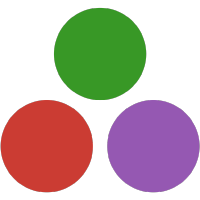
\includegraphics[height=1.4\fontcharht\font`\B]{julia_logo.png}%
}{Familiar}
%
%
\cvitemwithcomment{}{%
Clojure 
\includegraphics[height=1.4\fontcharht\font`\B]{Clojure_logo.png}, %
C, %
Bash 
\includegraphics[height=1.4\fontcharht\font`\B]{bash_logo.png}, %
Git 
\includegraphics[height=1.4\fontcharht\font`\B]{git_logo.png}%
}{Basics}
%
%
%
\section{Interests}
\cvitem{Music}{Jazz guitar, Trumpet}
\cvitem{}{Music theory and Jazz harmony}
\cvitem{}{Dance}
%
%
%
\clearpage
%
\end{document}
